\documentclass[12pt]{amsbook}
\usepackage{preamble}

\begin{document}
\pagenumbering{gobble} % This kills the page numbering

\begin{center}
   \textsc{\large MATH 271, Exam 1}\\
\end{center}
\vspace{1cm}

\noindent\textbf{Name} \; \underline{Solutions\hspace{6.5cm}}

\vspace{1cm}

\noindent\textbf{Instructions} \; No textbook, homework, calculators, phones, or smart watches may be used for this exam. The exam is designed to take 50 minutes and must be submitted at the end of the class period. All of your solutions should be easily identifiable and supporting work must be shown. You may use any part of this packet as scratch paper, but please clearly label what work you want to be considered for grading. Ambiguous or illegible answers will not be counted as correct.\\

\noindent\emph{Only the highest scoring \underline{five} problems will be counted towards your total score. You cannot get over 75 points.}

\vspace{1cm}

\begin{flushleft}
\textbf{Problem 1} \; \underline{\hspace{1cm}}/15

\vspace{.25cm}

\textbf{Problem 2} \; \underline{\hspace{1cm}}/15

\vspace{.25cm}

\textbf{Problem 3} \; \underline{\hspace{1cm}}/15

\vspace{.25cm}

\textbf{Problem 4} \; \underline{\hspace{1cm}}/15

\vspace{.25cm}

\textbf{Problem 5} \; \underline{\hspace{1cm}}/15

\vspace{.25cm}

\textbf{Problem 6} \; \underline{\hspace{1cm}}/15

\vspace{.5cm}

\textbf{Total} \;\hspace{1.1cm} \underline{\hspace{1.25cm}}/75
\end{flushleft}

\vspace*{4cm}


\begin{center}\large{There are extra pages between each problem for scratch work.\\

Please circle your answers!}\end{center}









% Problem 1
\newpage
\begin{problem}~\\

\def\arraystretch{2}% increase vertical spacing
\noindent\begin{tabularx}{\textwidth}{cXcc}
 & & T & F\\
(\theabc) & For any polynomial $p(z)=a_0 + a_1 z + \cdots +a_{n-1}z^{n-1}+a_{n}z^n$ there exists $n$ complex roots (possibly repeated). & \filledanswer & \answerbox\\
(\theabc) & Euler's formula is $e^{i\theta}=\sin \theta + i \cos \theta$. & \answerbox & \filledanswer\\
(\theabc) & $t=2$ is a solution to the differential equation $2x'=tx$. & \answerbox & \filledanswer\\
(\theabc) & All first order linear equations are separable. & \answerbox & \filledanswer\\
(\theabc) & The concentrations $A$ and $B$ for the chemical reaction \[A+B \xrightarrow{k} \textrm{Products}\] is modelled by the equations $\frac{dA}{dt}=-kB$ and $\frac{dB}{dt}=-kA$. & \answerbox & \filledanswer\\
(\theabc) & If $x_1$ and $x_2$ are solutions to a homogeneous linear equation, then the superposition $x=x_1+x_2$ is a solution as well. & \filledanswer & \answerbox\\
(\theabc) & All second order linear equations oscillate. & \answerbox & \filledanswer\\
(\theabc) & A solution $x(t)$ to an inhomogeneous second order linear equation is written as the sum $x=x_h+x_p$ where $x_h$ solves the homogeneous equation and $x_p$ is the particular integral.  & \filledanswer & \answerbox\\
(\theabc) & There are infinitely many states for the quantum particle in a 1-dimensional box. & \filledanswer & \answerbox\\
(\theabc) & States for the quantum particle in the 1-dimensional box can have any energy value. & \answerbox & \filledanswer\\
\end{tabularx}
\end{problem}



% Problem 2
\newpage
\begin{problem}
Let $z_1=-1+i$, $z_2=2-i$ and $z_3=2e^{i \pi}$.  
\begin{enumerate}[(a)]
    \item Plot and clearly label $z_1$, $z_2$, $z_1+z_2$, and $z_1\cdot z_2$ on the following graph.
    \begin{center}
    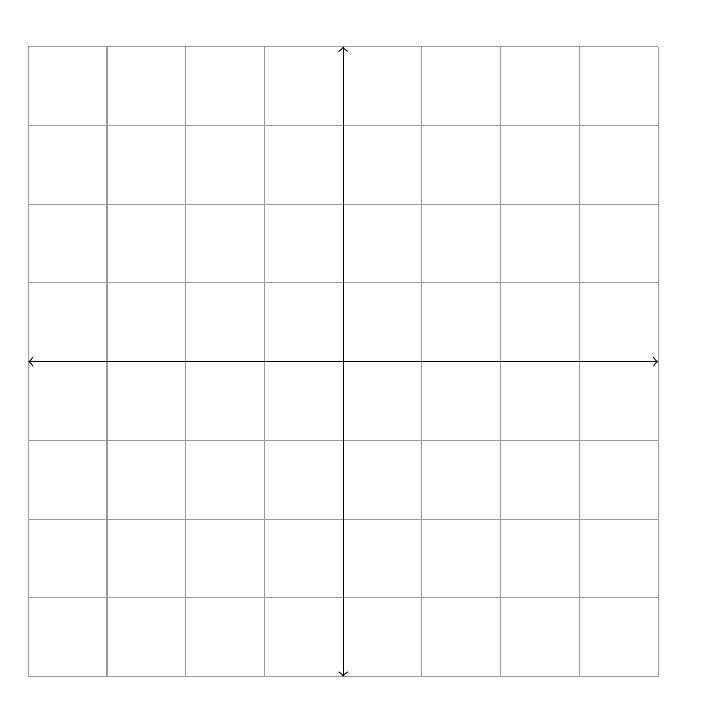
\begin{tikzpicture}[scale=1]
    \draw[thin,gray!80] (-4,-4) grid (4,4);
    \draw[<->] (-4,0)--(4,0) node[right]{$\RE$};
    \draw[<->] (0,-4)--(0,4) node[above]{$\IM$};
    
    \end{tikzpicture}
    \end{center}
    \vspace*{1cm}
    \item Compute $z_1^{-1}$ and $z_3^{-1}$.
    \vspace*{8cm}
    \item Write $z_3$ in Cartesian coordinates using Euler's Formula then plot and clearly label $z_3$ on the above graph.\\
    We can use the fact that $re^{i\theta}=\cos\theta + i \sin \theta$ to get
    \[
    2e^{i\pi} = 2\cos \pi + 2 \sin \pi = -2.
    \]
\end{enumerate}
\end{problem}

\newpage
\emph{Intentionally left blank to be used as scratch paper.}\\


% Problem 3
\newpage
\begin{problem}
The height above ground, $y(t)$, of a ball falling through air satisfies the differential equation
\[
y''=ky'-g,
\]
where $k$ and $g$ are positive constants.  
\begin{enumerate}[(a)]
    \item What is the order of this equation? Explain.
    \vspace*{3cm}
    \item Is this equation linear? Explain.
    \vspace*{3cm}
    \item Is this equation homogeneous or inhomogeneous? Explain.
    \vspace*{3cm}
    \item Let $k=0$ so we are left with
    \[
    y''=-g.
    \]
    What is the general solution to this new equation?
\end{enumerate}
\end{problem}

\newpage
\emph{Intentionally left blank to be used as scratch paper.}\\


% Problem 4
\newpage
\begin{problem}
The harmonic oscillator is given by the equation
\[
x''+ \frac{k}{m}x = 0.
\]
where $m$ is the mass of the oscillating object and $k$ is the spring constant.
\begin{enumerate}[(a)]
    \item Show that
    \[
    x(t)=A \cos\left(\sqrt{\frac{k}{m}}t\right).
    \]
    solves the initial problem with initial data $x(0)=A$ and $x'(0)=0$.
    \vspace*{6cm}
    \item Since this system has no damping, the total energy is \underline{conserved at all times}.  In particular, the total energy is given by
    \[
    E=\frac{1}{2}mx'(t)^2+\frac{1}{2}kx(t)^2 = \textrm{constant}.
    \]
    and is equal for all times $t\geq 0$. What is the total energy of the given particular solution $x(t)=A\cos\left(\sqrt{\frac{k}{m}}t\right)$?
    \vspace*{5cm}
    
\end{enumerate}
\end{problem}

\newpage
\emph{Intentionally left blank to be used as scratch paper.}\\


% Problem 5
\newpage
\begin{problem} For the following, explain in words how you could attempt to solve the following equations.  \emph{Hint: telling me the type of differential equation you're looking at helps!}
\begin{enumerate}[(a)]
    \item The equation
    \[
    x'+f(t)x=g(t).
    \]
    \vspace*{5cm}
    \item The equation 
    \[
    x'=f(x)g(t).
    \]
    \vspace*{5cm}
    \item The equation
    \[
    x''+bx'+cx=0.
    \]
\end{enumerate}
\end{problem}

\newpage
\emph{Intentionally left blank to be used as scratch paper.}\\


% Problem 6
\newpage
\begin{problem}
Schr\"odinger's equation was written as
\[
\left(-\frac{\hbar^2}{2m}\frac{d^2}{dx^2}+V(x)\right)\Psi(x)=E\Psi(x),
\]
where $V(x)$ is the potential at a point $x$, $E$ is the total energy, and $\Psi$ is the wave function.
\begin{enumerate}[(a)]
    \item For the free particle in a 1-dimensional box $[0,L]$, what are the boundary conditions for the wavefunction $\Psi$?
    \vspace*{3cm}
    \item Again, for the free particle in a 1-dimensional box, What is the potential inside of the box $(0,L)$?
    \vspace*{3cm}
    \item If a wavefunction $\Psi$ is normalized, then
    \[
    \int_0^L \|\Psi(x)\|^2dx=1.
    \]
    True or false?
    \vspace*{3cm}
    \item If our wavefunction $\Psi$ is normalized, how do we interpret the quantity
    \[
    P([a,b])=\int_a^b \|\Psi(x)\|^2dx?
    \]
    \vspace*{3cm}

\end{enumerate}
\end{problem}

\newpage
\emph{Intentionally left blank to be used as scratch paper.}\\

\end{document}  